% Label-shift knowability boundary (second per-family resolution of conj:gen).
% Numbers from scripts/labelshift_boundary_validation.py
% (results/theory/labelshift_boundary_validation.json).

A second family admits a complete characterization: \emph{label shift}, where the
class-conditionals are fixed and known from source while the target prior moves.

\begin{definition}[Evidence operator and label-shift reach]\label{def:lsreach}
Let $Y\in\{1,\dots,K\}$, class-conditionals $p(x\mid y)$ fixed (known from labeled
source), target prior $\pi\in\Delta_K$ unknown, and fixed maps $f_0,f_a$. The per-class
benefit $\delta_y=\E[\ell(f_0(X),Y)-\ell(f_a(X),Y)\mid Y{=}y]$ is source-computable and
$\Delta(\pi)=\delta\cdot\pi$ is affine. Let $M$ be the linear \emph{evidence operator}
mapping $\pi$ to the law of all label-free observables (the mixture, or any projection
of it such as a confusion matrix). The admissible ambiguity at $\pi$ is
$A(\pi)=(\pi+\ker M)\cap\Delta_K$, and the \emph{reach} is
$\rho(\pi)=\sup_{\pi'\in A(\pi)}|\delta\cdot(\pi'-\pi)|$.
\end{definition}

\begin{proposition}[Label-shift knowability boundary]\label{thm:ls-iff}
In the label-shift family, $\sign\Delta$ is label-free identifiable at $\pi$ \emph{if
and only if} $|\Delta(\pi)|>\rho(\pi)$. In particular:
\textup{(i)} if $M$ is injective on the simplex (e.g.\ linearly independent
class-conditionals, or an invertible confusion matrix), then $\rho\equiv0$ and the
decision is identifiable whenever $|\Delta|>0$; committing
$\sign(\delta\cdot\widehat\pi)$ iff $|\delta\cdot\widehat\pi|>\rho+\varepsilon_n$ (any
consistent estimator $\widehat\pi$ of a point of $A(\pi)$ with radius $\varepsilon_n$)
wrong-commits with probability at most $\alpha$ against every admissible prior.
\textup{(ii)} If $|\Delta(\pi)|<\rho(\pi)$, the admissible segment
$\{\pi+tv\}\subset A(\pi)$ along a null direction $v\in\ker M$ realizes both signs of
$\Delta$ while \emph{all} label-free observables --- the unlabeled target law and the
labeled source --- coincide: the pair instantiates Theorem~\ref{thm:imp} inside the
family, and the regime is unknowable.
\end{proposition}
\begin{proof}
$\Delta$ is affine on the compact convex set $A(\pi)$, so
$\{\Delta(\pi'):\pi'\in A(\pi)\}$ is the interval
$[\Delta(\pi)-\rho,\,\Delta(\pi)+\rho]$ with the supremum attained.
(i) On the $1-\alpha$ event the estimate lands within $\varepsilon_n$ of a member of
$A(\pi)$; if $|\delta\cdot\widehat\pi|>\rho+\varepsilon_n$ then every member of
$A(\pi)$ --- in particular the truth --- has benefit of the committed sign.
(ii) If $|\Delta(\pi)|<\rho$ the interval straddles $0$; pick
$t_\pm$ with $\Delta(\pi+t_\pm v)$ of opposite signs ($t\mapsto\Delta(\pi+tv)$ is
affine, hence onto the interval). Worlds $\pi$ and $\pi+tv$ share the observable law by
$v\in\ker M$ and share the source by construction; apply Theorem~\ref{thm:imp}.
\end{proof}

\begin{proposition}[Reach is monotone in evidence]\label{prop:reach-mono}
If evidence is enlarged, $M\mapsto M'$ with $\ker M'\subseteq\ker M$, then
$\rho'(\pi)\le\rho(\pi)$ for every $\pi$: richer label-free evidence can only shrink
the unknowable region.
\end{proposition}
\begin{proof}
$A'(\pi)=(\pi+\ker M')\cap\Delta_K\subseteq A(\pi)$, and the supremum over a subset is
no larger.
\end{proof}

\noindent\emph{Numerically validated}
(\texttt{labelshift\_boundary\_validation.py}; Fig.~\ref{fig:lsboundary}). With three
distinct Gaussian class-conditionals (injective $M$): zero false certifications over
$30$ random priors. With classes $2,3$ \emph{identical} (singular $M$, null direction
$v=(0,1,-1)/\sqrt2$): paired worlds $\pi$ and $\pi+tv$ are statistically
indistinguishable (two-sample KS $p=0.051$ on $3\times10^4$ draws); the certificate
that commits only when the whole admissible benefit interval has one sign made
\emph{zero} false certifications over $40$ priors; genuine sign flips occur inside the
reach interval whenever it straddles zero (the converse is realized, not hypothetical);
the interval endpoints are attained exactly (tightness gap $<10^{-9}$); and adding a
class-separating feature shrinks the reach from $0.156$ to $0$
(Proposition~\ref{prop:reach-mono} in action).

\begin{figure}[t]\centering
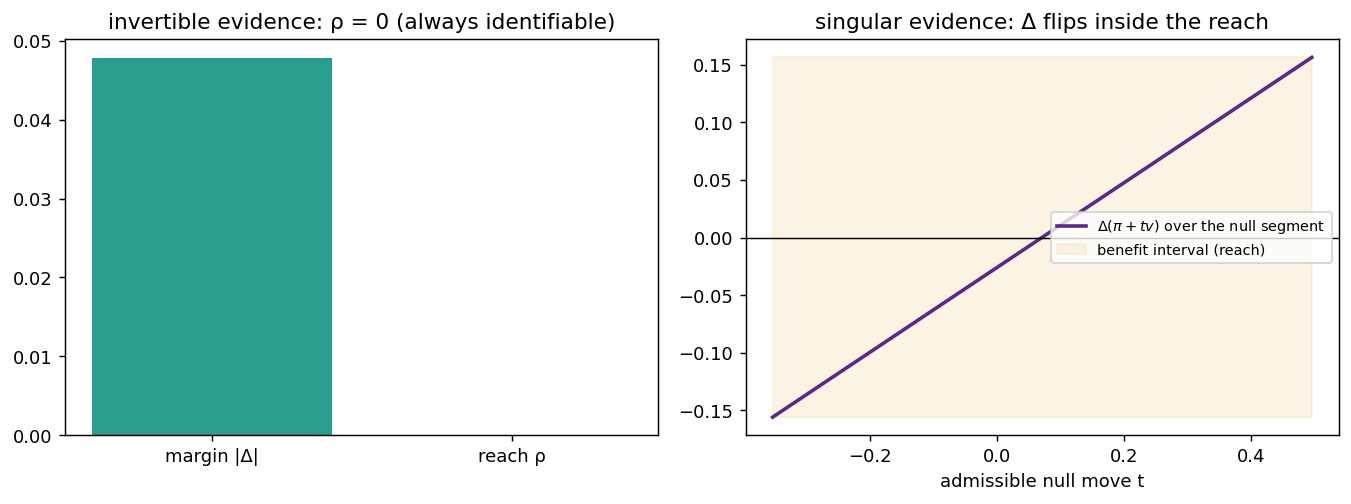
\includegraphics[width=0.92\linewidth]{figures/fig_labelshift_boundary.png}
\caption{The label-shift boundary (Proposition~\ref{thm:ls-iff}). Left: injective evidence
operator, reach $0$ --- always identifiable. Right: singular evidence; the benefit
$\Delta(\pi+tv)$ sweeps the reach interval along the unobservable null segment and
crosses zero --- identifiable exactly when the margin clears the reach.}
\label{fig:lsboundary}
\end{figure}

\paragraph{Weight (honest).} The identifiability machinery is classical (label-shift
estimation \`a la BBSE); the new content is the \emph{decision-level} iff --- margin
versus a null-space reach, with the converse constructed inside the family via
Theorem~\ref{thm:imp} --- and the monotonicity of the reach in the evidence. The
known-conditional assumption does the work and is stated as such; unknown or drifting
class-conditionals re-enter the open general case of Conjecture~\ref{conj:gen}.
